% Section content template for individual Educative lessons
% This file contains the actual content for a specific section
% Generated from Educative API section content

% Section: Introduction to the Payment System
% Section ID: 5914042189086720
% Section Slug: introduction-to-the-payment-system
% Generated: 2025-12-08T15:30:57.363115

In today's digital age, financial technology (fintech) is reshaping the landscape of e-commerce and digital marketing. Seamlessly connecting merchants and consumers, fintech enables transactions to happen with just a few clicks, making purchases faster, more convenient, and increasingly secure. Innovations like integrated payment platforms, digital wallets, and fintech-driven gateways are not only enhancing the customer experience but also streamlining business operations.
\\
In this lesson, we'll explore how digital payment systems work and their pivotal role in powering modern commerce.

\subsection{What is a digital payment system?}\label{6JtsN4LBgDbI8LUC_UPQp}
\\
A \textbf{payment system} is a mechanism or process that enables individuals, businesses, and organizations to transfer money or make transactions for the purpose of making a purchase. It encompasses various methods and technologies, both digital and traditional, that facilitate the exchange of money or goods. Payment systems encompass a wide range of transactions, including credit and debit card transactions, bank transfers, electronic funds transfers (EFTs), mobile payments, digital wallets, and cryptocurrencies. These systems ensure secure and efficient financial transactions between parties, supporting commerce and economic activities on various scales.
\\
In this design problem, we'll focus on payments made through credit and debit cards.
\\
Let's first understand the payment process in detail before moving to any aspect of the payment System Design.

\subsection{The payment process}\label{vCPKyd9_GLSVbGtqsD0n_}
\\
Multiple entities are involved in the payment process. Assume that a customer wants to pay for goods or services using a credit or debit card. First , they have to enter their credit or debit card details to pay online. However, this complex process entails multiple steps and interacting entities, including cardholder verification, payment processing and validation, and merchant registration.
\\
The following figure illustrates the flow of a payment processing system:

\begin{figure}[htbp]
 \centering
 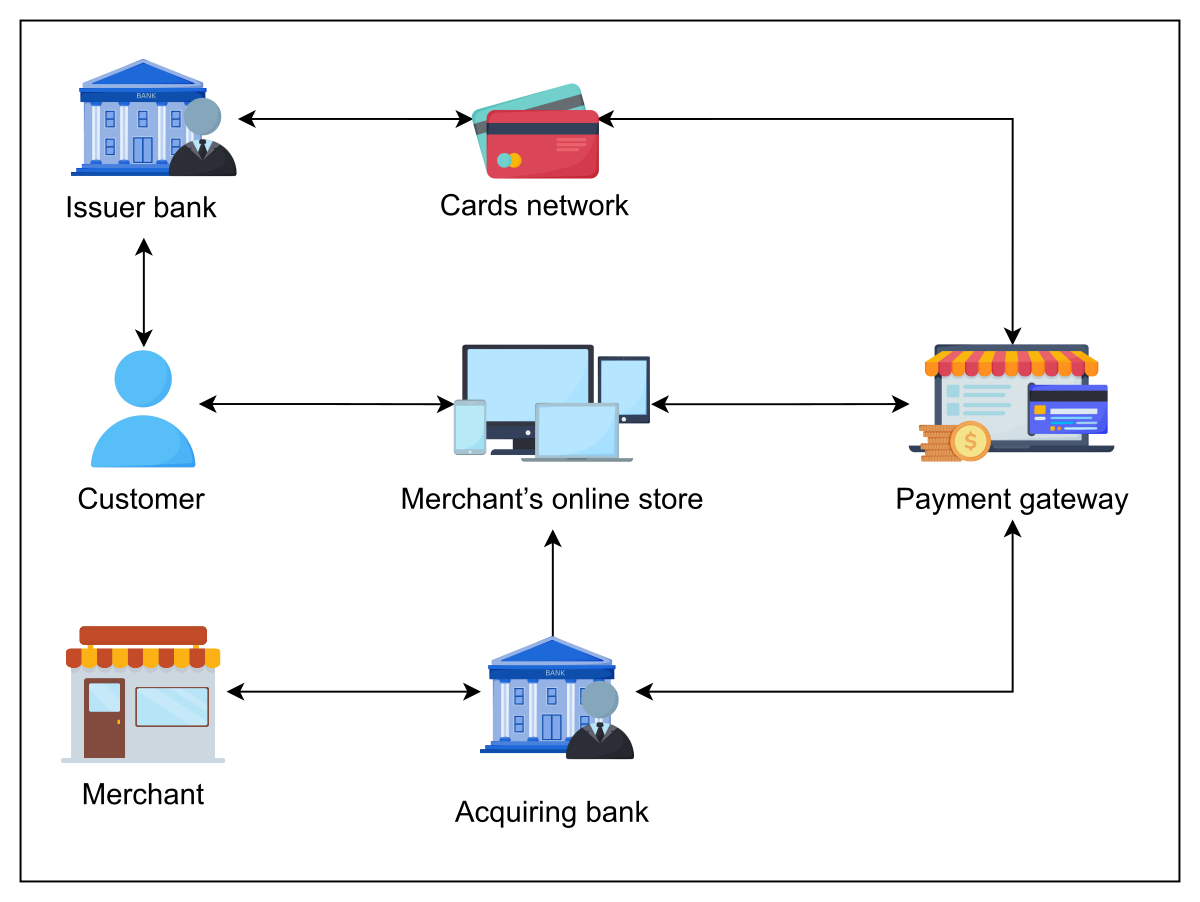
\includegraphics[width=0.5\textwidth]{Images/chapter_40/section_5914042189086720/6057695698092032.png}
 \caption{Payment processing system and the entities involved in it}
\end{figure}

The role of different entities involved in the payment processing system is mentioned in the following table:

\begin{table}[htbp]
\centering
\small
\adjustbox{max width=\textwidth}{
\begin{tabular}{|p{0.250\textwidth}|p{0.700\textwidth}|}
\hline
\textbf{Entities} & \textbf{Description} \\
\hline
\hline
Customer & \begin{itemize} \tightlist \item A cardholder who wants to purchase goods or services. \end{itemize} \\
\hline
Merchant & \begin{itemize} \tightlist \item A company or person who provides goods or services. \end{itemize} \\
\hline
Issuer bank & \begin{itemize} \tightlist \item The bank that holds the customer\emph{'s} account and provides credit or debit cards. \end{itemize} \\
\hline
Acquiring bank & \begin{itemize} \tightlist \item The bank holding the merchant's account. \end{itemize} \\
\hline
Merchant\textquotesingle s online store & \begin{itemize} \tightlist \item The online website where the customer purchases goods or services by providing credit card details. \end{itemize} \\
\hline
\hfill\break Payment gateway & \begin{itemize} \tightlist \item A network that facilitates and authorizes transactions of funds to merchants' accounts. \item Requests and receives payment from the customer's account. \end{itemize} \\
\hline
\hfill\break Cards network & \begin{itemize} \tightlist \item Validates the credit or debit card information. \item Facilitates payments via credit and debit cards. \item Sets the terms for credit or debit card transactions. \end{itemize} \\
\hline
\end{tabular}
}
\end{table}

In a payment system, especially for credit card transactions, the process typically involves two key phases: \emph{authorization} and \emph{settlement}. These phases ensure that a transaction is authorized and then completed by transferring funds from the customer's account to the merchant's account. The following is an overview of each phase:

\subsubsection{The authorization phase}\label{m_sVjP3-kC8zVKg6r8TKw}
\\
The authorization phase is the initial step in a payment transaction. Its primary purpose is to verify whether the customer's payment method (e.g., credit card) is valid, has sufficient funds or credit available, and can be used to make the intended purchase.

\begin{enumerate}
\item
\protect\phantomsection\label{aJNzabO1gkrC_2LDQ06Tw}
The customer initiates a payment by providing payment details, such as credit card information, to the merchant's payment system (usually via a payment gateway).
\item
\protect\phantomsection\label{QOJsZvKFiEoIRPRnGxDTj}
The payment gateway sends the payment request to the customer's issuer bank (the bank that issued the credit card).
\item
\protect\phantomsection\label{Q1U4m0ry0-wulniV2Ecft}
The issuer bank performs several checks, including verifying the card's validity, checking for available credit, and ensuring the transaction is not fraudulent.
\item
\protect\phantomsection\label{qQ8aBmO9FVfY5xnnrw9G4}
If all checks pass successfully, the issuing bank sends the authorization code to the payment gateway, indicating that the transaction is approved.
\item
\protect\phantomsection\label{BWDoaz1OBY07OhgNSFed1}
The payment gateway relays the authorization code to the merchant, indicating that the customer's payment method has been authorized for the transaction.
\end{enumerate}
\\
If the authorization is successful, the transaction amount is reserved on the customer's credit card but not transferred to the merchant. The funds are held pending until the settlement phase.

\subsubsection{The settlement phase}\label{k-bOJasmnmRB0SLbhKTmW}
\\
The settlement phase occurs after the authorization phase. It finalizes the payment transaction by transferring the authorized funds from the customer's account to the merchant's.

\begin{enumerate}
\item
\protect\phantomsection\label{RJ7zyp2EdvFj7qJxT4uop}
After receiving the authorization code, the merchant accumulates authorized transactions for a certain period (for example, a day's worth).
\item
\protect\phantomsection\label{_E2TbSSgV2A8DqPsxJtwY}
The merchant initiates a batch settlement process, sending all authorized transactions to the payment processor or acquiring bank. In some cases, a payment gateway also functions as a payment processor. For example, Stripe is a payment gateway and a payment processor.
\item
\protect\phantomsection\label{EqsdNUWCJmrCM1U-R9Y4y}
The payment processor or acquiring bank verifies the transactions and transfers funds from the customers' issuing banks to the merchant's bank.
\item
\protect\phantomsection\label{hunmcOI2ETzQLK6vuRJve}
The acquiring bank or payment processor reconciles the transactions, ensuring all authorized transactions are accounted for and the correct funds are transferred.
\item
\protect\phantomsection\label{iFrn5GQFcf4nQaME7dC9l}
Once reconciliation is complete, the acquiring bank or payment processor deposits the funds into the merchant's bank account, completing the settlement process.
\end{enumerate}
\begin{quote}
\textbf{Note:} The authorization and settlement phases may not occur simultaneously. Authorization is typically immediate and confirms that a valid payment method and funds are available. On the other hand, settlement may occur in batches and is the process of moving the funds to the merchant's account in a bulk transfer.
\end{quote}
\\
During the settlement phase, the authorized funds are transferred to the merchant's account, and the payment transaction is considered complete. The customer's credit card statement will reflect the finalized transaction.
\\
In what scenarios could authorization succeed but settlement fail, and how should the system handle it?
\\
Use the AI assessment widget below to submit your solution and get an interactive response.

\textbf{Question:}

The settlement phase

\textbf{Reference Answer:}

Failures can occur due to network issues, bank errors, or insufficient funds at settlement; the system should detect the failure, notify stakeholders, and attempt retries or reversal.

We have explored how the payment processing system works. Now, let's move on to design a payment system by considering the following requirements:

\subsection{Requirements}\label{qsT7Ul-rpKucK8X_aHMnv}
\\
Let's understand the functional and non-functional requirements of the payment system.

\subsubsection{Functional requirements}\label{oMpJfx6XOSdl_oFZbhbAM}
\\
We are designing a payment system to accept credit or debit card payments via a PSP(Payment service provider). Therefore, we will stick to the following functional requirements:

\begin{itemize}
\item
\protect\phantomsection\label{97Cs178IPkL1pqJ9aiJ-Y}
\textbf{User registration and authentication:} Users should be able to create accounts, log in securely, and reset passwords.
\item
\protect\phantomsection\label{K-mlfx3vw_-geXIhiVSHd}
\textbf{Payment processing:} Users should be able to initiate payment processing upon purchasing a product or service. The system should accept payment via credit and debit cards.
\item
\protect\phantomsection\label{wenot0SHXd32tupmQX__l}
\textbf{Transaction history:} Users should be able to view a history of their transactions, including dates, amounts, and descriptions.
\item
\protect\phantomsection\label{m1PbJBFmq7m7a8RdVMwHs}
\textbf{Balance management:} Users should be able to check their account balances, including available funds and pending transactions.
\item
\protect\phantomsection\label{1LUI1RJnrhLUC2AChHA0k}
\textbf{Mobile accessibility:} Users should be able to access and use the payment system through mobile apps or responsive web interfaces.
\end{itemize}

\subsubsection{Non-function requirements}\label{5LDiKiJczmlXpnrSIL_8H}
\\
The following are the non-functional requirements that the payment system should meet for smooth operations:

\begin{itemize}
\item
\protect\phantomsection\label{mvXDeOk-So9A7oMDj9eAd}
\textbf{Data integrity and security:} The system should comply with industry security standards. It should also have robust data encryption and secure storage mechanisms, maintain consistency, and prevent data corruption.
\item
\protect\phantomsection\label{6fqK_ilNjAkQm9ZHvHewD}
\textbf{Availability:} The system should be highly available to ensure users can always access it.
\item
\protect\phantomsection\label{o5kV5u6cHfpuoCh2-cgYK}
\textbf{Reliability:} Redundancy, failover mechanisms, and backup systems should be in place.
\item
\protect\phantomsection\label{dLDrtspGxL9UaVSYwmziA}
\textbf{Scalability:} The system should scale seamlessly as the user base and transaction volume grow. It should also handle peak loads during events like promotions or sales.
\item
\protect\phantomsection\label{p1b3kcMs5u6yrBe69Y0L-}
\textbf{Performance:} The system should be able to handle high transaction loads without experiencing significant slowdowns. The response times for payment processing and account updates should also be within acceptable limits(Payment processing and account updates should occur within a few seconds to ensure a smooth and responsive user experience. Ideally, transactions are completed in under 3 seconds, with account changes reflected instantly or within moments to maintain user trust and system reliability.).
\end{itemize}
\\
Based on the requirements, we'll estimate the required resources for our system as follows:

\subsection{Resource estimation}\label{x-oG0xpEFY_nG9yTexRDf}
\\
For resource estimation, we assume that our system can perform 50 million transactions per day, or 2 million transactions per hour. This number could increase to 5 million transactions per hour in peak hours. Assuming these numbers, let's estimate the storage, bandwidth, and required number of servers.

\subsubsection{Storage estimation}\label{ari1tNUi6WaRjGANC9cac}
\\
In the payment system, we need to store various types of data, including users' details and their associated payment information. Also , we would be required to store transaction records. Assume that each transaction takes 100 bytestransaction and each user's record takes up to 200 bytesuserrecord. So
, the storage required per day would be as follows:

\[
\text{Storage required per day} = \text{50 M} \times100 \text{ bytes}+ \text{200 bytes} \approx 5 \text{ GB}
\]

\begin{quote}
\textbf{Note:} Since each user\textquotesingle s record is stored only once and transactions only reference the user ID, the 200 bytes are not repeated across the 50 million transactions.
\end{quote}
\\
Below is a calculator to help us estimate our required storage.~


\subsubsection{Bandwidth estimation}\label{1J5zYYTquENBn5MRtFx7h}
\\
In a payment system,~bandwidth~ensures timely and reliable communication between clients, the payment gateway, and external systems like banks or PSPs. Each transaction involves data moving~into~and~out of~the system, requests sent to process payments, and responses returned with confirmation, status, and audit details. Let 's estimate the incoming and outgoing bandwidths for our system:
\\
\paragraph{Incoming bandwidth}\label{l1OIoYpXD1vJew_aJf7R8}
\\
As mentioned earlier, our system is designed to support up to 5 million transactions per hour during peak periods. In other words, our system should be capable of handling approximately 1400 transactions per second. Given that the size of each transaction is 100 bytes, which can be calculated as:

\begin{aligned}
\text{Total}_{\text{incoming bandwidth}}
&= \text{Total}_{\text{transactions/sec}} \times \text{Total}_{\text{transaction size}} \\
&= 1400 \times 100\ \text{Bytes} \\
&\approx 1.12\ \text{Mbps}
\end{aligned}


\paragraph{Outgoing bandwidth}\label{IW3B-sEAPPaThanO29qCf}
\\
The outgoing response typically contains more information, including status, authorization tokens, timestamps, messages, and optional fields such as digital signatures or audit references. On average, we assume~130 bytes(Assumed based on fields such as transaction ID (16 bytes), status code (10 bytes), timestamp (8 bytes), user ID (16 bytes), and metadata or protocol overhead (\textasciitilde80 bytes).)~per response.

\begin{aligned}
\text{Total}_{\text{outgoing bandwidth}}
&= \text{Total}_{\text{responses/sec}} \times \text{Total}_{\text{response size}} \\
&= 1400 \times 130\ \text{Bytes} \\
&\approx 1.46\ \text{Mbps}
\end{aligned}


We can use the following calculator to estimate the incoming and outgoing bandwidths:

\subsection*{Quiz}
\vspace{0.3cm}
\noindent
\textbf{Question 1:} Assume that the number of transactions is increased to 3000 per second in peak time. Also
, suppose that each transaction's size is increased to 350 bytes. What would be the bandwidth requirement estimation in this case?
\\[0.2cm]
\begin{itemize}
 \item \textbf{[CORRECT]} {{\(8400 \ Kbps\)}}
\\[0.1cm]
\textit{Explanation:} 
{{\((3000\times350\times8)/1000=8400 \ Kbps\)}}
 \item {{\(8400 \ KBps\)}}
 \item {{\(8.4 \ Kbps\)}}
 \item None of the above
\end{itemize}

\begin{quote}
\textbf{Note:} Keep in mind that these estimations are fairly basic, and in a real-world situation, we would probably have to consider extra factors like redundancy, backups, indexing, and other metadata.
\end{quote}
\subsubsection{Number of servers estimation}\label{HvVH3xMBaehVtQnAQeQwi}
\\
To estimate the number of servers, we need to know the number of daily active users of the payment system. We assume that our system can perform 50 million transactions per day (50 million daily active users). Considering
\href{https://www.educative.io/courses/grokking-the-system-design-interview/put-back-of-the-envelope-numbers-in-perspective}{our assumption} of using daily active users as a proxy for the number of requests per second, we get 50 million requests per second. Then
, we use the following formula to calculate the number of servers:

\[
\text{Servers needed at peak load = }\frac{\text{Number\ of\ requests/second}}{\text{RPS of server}}
\]

Using 64,000 as an estimated RPS a server can handle, the required servers are estimated as follows:

\[
\text{Servers needed at peak load =} \frac{\text{50 million}}{\text{64,000}} ≈ \text{782 servers}
\]

\begin{figure}[htbp]
 \centering
 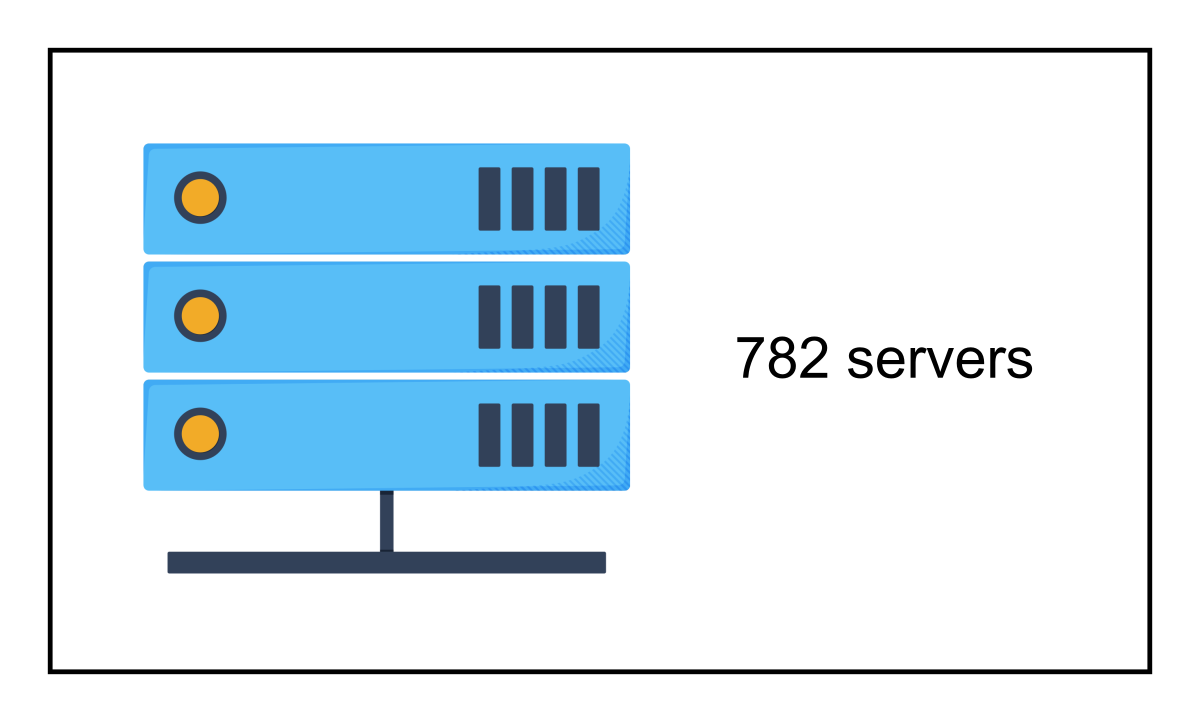
\includegraphics[width=0.15\textwidth]{Images/chapter_40/section_5914042189086720/5686815434342400.png}
 \caption{Number of servers required for payment system}
\end{figure}

After discussing the required resources, let's move on to the building blocks we'll use to design the payment system.

\subsection{Building blocks we will use}\label{eCIEHWViMEH_zSU1IGXy_}
\\
When designing a payment system, we will use the following building blocks. We would also need other essential components and services, including a payment gateway, risk check service, and reconciliation system.

\begin{figure}[htbp]
 \centering
 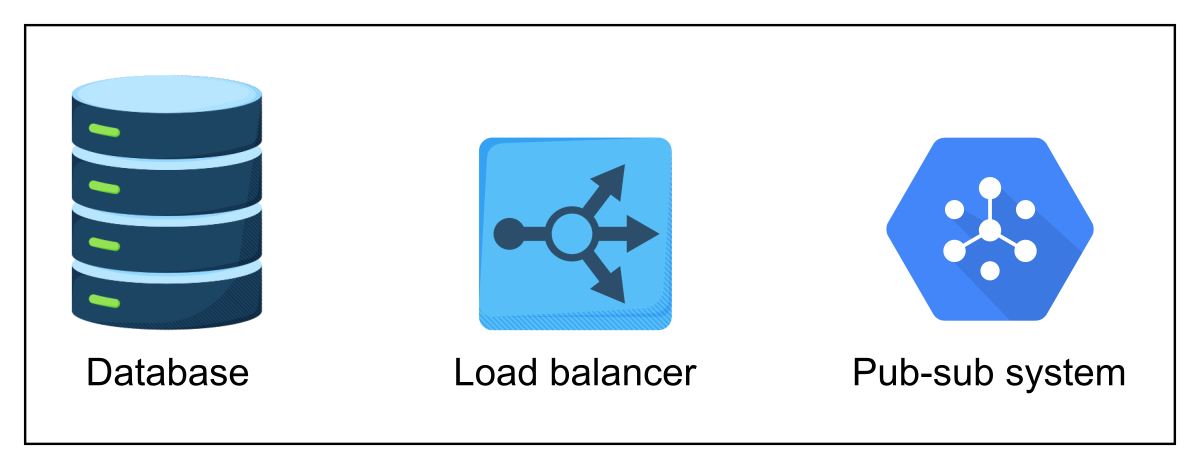
\includegraphics[width=0.5\textwidth]{Images/chapter_40/section_5914042189086720/4640594854805504.png}
 \caption{Building blocks in the payment System Design}
\end{figure}

\begin{itemize}
\item
\protect\phantomsection\label{SoJXSLGRlKpfGVIutZDHy}
\href{https://www.educative.io/courses/grokking-the-system-design-interview/introduction-to-databases}{\textbf{Databases}}~are required to store user-generated payment events and transaction data.
\item
\protect\phantomsection\label{ku0zVqQPIuzZkC2Drf6wB}
\href{https://www.educative.io/courses/grokking-the-system-design-interview/introduction-to-load-balancers}{\textbf{Load balancers}}~must distribute millions of incoming user requests among available servers.
\item
\protect\phantomsection\label{GKKiCEVEw7-rr637G73VC}
\href{https://www.educative.io/courses/grokking-the-system-design-interview/system-design-the-pub-sub-abstraction}{\textbf{Pub-sub systems}} decouple essential services such as the payment service, wallet, and ledger services.
\end{itemize}
\\
In the next lesson, we'll focus on the design of a payment system.

% End of section content